\section{Autonómne vozidlá}\label{sec:AutonomneVozidla}
\subsection{Čo je to autonómne vozidlo?}
\acrfull{av}, niekedy nazývané aj samoriadiace auto je dopravný prostriedok, ktorý, na rozdiel od tradičných vozidiel nevyžaduje vodiča. Autonómne vozidlá vykonávajú túto úlohu pomocou viacerých hardvérových a softvérových systémov. Hoci ani v roku 2026 nemá termín 'samoriadiace' jednotnú štadardnú definíciu, hlavným cieľom týchto technológií zostáva eliminácia ľudských chýb, zvýšenie efektivity premávky a sprístupnenie prepravy ľudom, ktorí nie sú schopní šoférovať sami.\par
Na vnímanie okolia vozidla používame senzory detekcie objektov. Systém vnímania používa kamery, \acrfull{radar}, \acrfull{lidar} a ultrazvukové senzory, pričom každý z nich má špecifickú funkciu. Autonómne vozidlá často pracujú s čiastočne neznámym a dynamickým prostredím, preto si musia vystavať model svojho prostredia a zároveň sa v ňom lokalizovať. Tento proces je známy pod skratkou SLAM (súčasná lokalizácia a mapovanie). Spočíva v spracovaní dát zo senzorov, máp a systéme \glslink{gps}{globálneho polohovacieho systému} \acrshort{gps}, vďaka čomu si zariadenie vytvorí model prostredia a určí v ňom svoju polohu v reálnom čase~\cite{wevolver2020}.\par
Tretí systém je zodpovedný za plánovanie a rozhodovanie. Na základe dát z predchádzajúcej vrstvy vozidlo vyhodnocuje a reaguje na vývoj dopravnej situácii. Táto vrstva má mnoho funkcií od plánovania trasy po vyhýbanie sa prekážkam. Najčastejšie sa používajú modely strojového učenia, vrátane neurónových sietí.\par
Posledným kľúčovým článkom je konanie a ovládanie. Systém ovládania vozidla premení abstraktné požiadavky predchádzajúcej vrstvy na fyzické pohyby auta. Zodpovedá za smerové riadenie, zrýchľovanie a brzdenie. Pokročilé algoritmy zároveň zabezpečujú, aby pohyb bol plynulý, stabilný a rešpektoval limitácie podvozku. Vďaka integrácii týchto systémov dokáže autonómne vozidlo navigovať v komplexných dopravných situáciách s minimálnou až nulovou potrebou ľudského zásahu.
\subsection{Úrovne autonómnych vozidiel}
Úrovne autonómnych vozidiel sú definované organizáciou SAE International v štandarde SAEJ3016. Tento dokument delí automatizáciu riadenia do šietstich stupňov (0-5) podľa toho, akú časť jazdy zabezpečuje systém a akú úlohu ešte stále zohráva vodič. O samoriadiacich autách sa často hovorí ako o jednej kategórii, no v praxi ide o postupný vývoj od minimálnej podpory riadenia až po úplnú autonómiu vozidla bez zásahu človeka~\cite{saej3016}.
\subsubsection{Úroveň 0}
\paragraph{Žiadna automatizácia}Na tejto úrovni všetky činnosti vykonáva ľudský vodič. Vozidlo môže mať bezpečnostné systémy, ako napríklad upozornenie opustenia jazdného pruhu, no samotné riadenie je plne v rukách človeka.
\subsubsection{Úroveň 1}
\paragraph{Asistované riadenie}Systém pomáha s postranným alebo pozdĺžnym riadením vozidla ale nie v obidvoch prípadoch naraz. Sem patria asistencie ako udržiavanie rýchlosti (tempomat) alebo mierne korigovanie smeru. Vodič však musí neustále sledovať situáciu na vozovke a mať ruky na volante.
\subsubsection{Úroveň 2}
\paragraph{Čiastočná automatizácia}Vozidlo dokáže súčasne riadiť smer aj rýchlosť, stále však platí, že vodič nepretržite dohliada na jazdu a je pripravený zasiahnuť v prípade núdze. Systém vykonáva viac úloh riadenia naraz, no zodpovednosť upadá na človeka.
\subsubsection{Úroveň 3}
\paragraph{Podmienená automatizácia}Jazda v špecifickej situácii je automatizovaná a vodič nemusí aktívne sledovať okolie. Ak však systém vyhodnotí, že situáciu nezvládne, kontrola vozidla sa vráti vodičovi. Vodič musí byť pripravený prevziať kontrolu nad vozidlom.
\subsubsection{Úroveň 4}
\paragraph{Vysoká automatizácia}Na tejto úrovni je vozidlo schopné zvládnuť jazdu úplne samo v rámci definovaných prostredí alebo podmienok. V prípade, že sa vozidlo dostane mimo týchto podmienok, dokáže bezpečne zastaviť. Prítomnosť ľudského šoféra nie je nutná.
\subsubsection{Úroveň 5}
\paragraph{Plná automatizácia}Najvyšší stupeň automatizácie, vozidlo dokáže jazdiť samostatne za všetkých podmienok, v ktorých dokáže jazdiť človek. Neexistuje potreba vodiča. Vozidlo zastaví v prípade zlyhania určitých modulov riadenia.

\section{Analýza súčasného stavu}\label{sec:Analyza}
\subsection{Aktuálny stav technológie}
V posledných rokoch sme zaznamenali nárast vydaní automobilov tretej úrovne autonómnosti, autonómne taxi služby sa stávajú realizovateľným spôsobom dopravy v mestách a dostali sme prvé ukážky kamiónov bez nutnosti ľudského vodiča~\cite{electronics2022}\cite{mckinsey2026}.\par
Vďaka vývoju v oblasti umelej inteligecie a zvýšenia výkonu výpočtových platforiem sme zaregistrovali značný pokrok v technológiách autonómnych vozidiel. Výrobcovia sa snažia zlepšovať kombinácie \acrshort{radar}ových, \acrshort{lidar}ových a kamerových dát tak, aby boli robustnejšie voči dopravným a poveternostným podmienkam. Pokračuje snaha v návrhu scenárov pre hraničné sitúacie, čím sa zlepší percepčná schopnosť autonómnych systémov a zrýchli ich nasadenie~\cite{motortrend2026}\cite{nvidia2026}.\par
Autonómne vozidla zaznamenali značnú investíciu ale aj kontrolu zo strany štátnych a nadnárodných organizácií. Spoločnosti, ktoré poskytujú služby samoriadiacich vozidiel rozširujú svoju dostupnosť, znižujú počet senzorov a náklady na hardvér. Hoci technológický pokrok napreduje, integrácia do infraštruktúry mesta zostáva podstatnou výzvou pre adopciu \acrshort{av} do dopravy. Štandard SAE International preto opisuje plán prechodu od asistencie šoférovania po plne autonómnu prevádzku~\cite{theguardian2026}\cite{waymo2026}.
\subsubsection{Umelá inteligencia}
\acrfull{ai} vykonáva dôležitú funkciu v percepčnom, rozhodovacom a plánovacom systéme autonómneho vozidla, čím nahrádza rolu ľudského vodiča. Moderné systémy používajú strojové učenie (machine learning) na detekciu hazardov na ceste, klasifikáciu dopravných značiek a sledovanie a predikciu pohybu chodcov a ostatných vozidiel~\cite{hamza2023}.\par
V súčasnosti sa autonómne modely trénujú na obrovskom množstve anotovaných obrázkov, videí, simulácií a skutočných jazdných dát, aby v praxy zvládli širokú škálu scenárov. Hlboké učenie (deep learning) a učenie posilňovaním (reinforcement learning) sa používajú v novodobých autonómnych vozidlách. Deep learning, podskupina strojového učenia, pracuje na princípe viacvrstvových neurónových sietí, čím sa fungovaním podobá ľudskému mozgu. Reinforcement learning mení správanie modelu využitím systému odmien a penalizácií~\cite{grigorescu2019}.\par
Napriek značnej komplexnosti zostáva riešenie hraničných prípadov (edge cases)  zásadnou výzvou pre dnešné systémy. Potreba veľkého množstva tréningových dát a vysoká hranica bezpečnosti a spoľahlivosti výrazne spomaľuje nasadenie vozidiel do reálnej premávky.
\subsubsection{Senzory}
Senzory sú spôsob akým autonómne vozidlá vnímajú svoje okolie. Ako je možné vidieť na obrázku \ref{fig:sensors}, v súčasnosti sa v autách využíva kombinácia kamier, \acrshort{lidar}ových, \acrshort{radar}ových a ultrazvukových senzorov~\cite{badue2021}.\par
\begin{figure}[!ht]
	\centering
	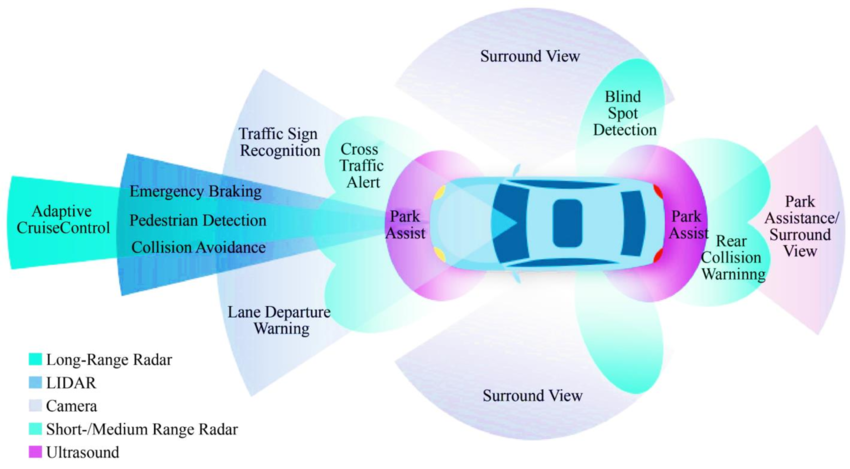
\includegraphics[scale=1.50]{img/sensors.png}
	\caption{Ako \acrshort{av} vnímaju prostredie}
	\footnotesize{\cite{hamza2023}, licencované pod CC BY 4.0.}
	\label{fig:sensors}
\end{figure}
Kamery predstavujú najrozšírenejší typ senzorov; sú nákladovo efektívne, no citlivé na zlé osvetlenie a počasie. Používajú sa na detekciu jazdných pruhov, rozpoznávanie dopravných značiek a identifikáciu chodcov a vozidiel. \acrshort{radar} využíva elektromagnetické vlny na meranie vzdialenosti a rýchlosti. Používa sa najmä pre detekciu vzdialených objektov aj v nepriaznivých poveternostných podmienkach (dážď, hmla, sneh). \acrshort{lidar} používa laserové impulzy na vytvorenie detailného trojrozmerného modelu okolia, no okrem vysokých nákladov je aj viac náchylný na zlé počasie. Ultrazvukové senzory majú využitie v detekcii objektov na krátke vzdialenosti, napríklad pri parkovacích manévroch.\par
Súčasný vývoj v oblasti senzorov sa zameriava primárne na zvyšovanie presnosti meranie, optimalizovanie počtu potrebných senzorov a výrazné znižovanie ich ceny. Výrobcovia taktiež zefektivňujú kombinovanie dát viacerých senzorov, tzv. senzorovú fúziu, čím zvyšujú presnosť a spoľahlivosť systému.
\subsection{Použitie autonómnych vozidiel}
Autonómne vozidlá ponúkajú široké spektrum využitia, pričom ich možnosti sa v posledných rokoch rozširujú. K najpozoruhodnejším oblasťiam ich využitia patrí doprava. Hlavným cieľom je zvýšiť bezpečnosť a plynulosť premávky. Ďalšie využitie je v logistike tovaru, kde nahrádzajú rutinnú manuálnu prácu tradične vykonávanú ľudmi.\par
\subsubsection{Autonómne taxi služby}
Autonómne taxi služby, často nazývané robo-taxíky predstavujú jednu z najpokročilejších foriem využitia autonómnych služieb. Proces od objednania, naplánovania trasy po prepravy pasažierov je plne automatizovaný. Mnohí výrobcovia automobilov, technologícké spoločnosti a štátne organizácie investujú zdroje do vývoju robo-taxíkov. Na popredí je firma Waymo, ktorá je dcérskou spoločnosťou Alphabet. Ich automobily, ktoré spĺňajú štvrtú úroveň autonómie, využívajú \acrshort{lidar}, \acrshort{radar} a kamery na vytvorenie trojrozmerného obrazu prostredia. S každou ďalšou generáciou vozidiel redukujú počet senzorov, čím znižujú náklady na výrobu a zlepšujú škálovateľnosť projektu.\par
Alternatívny prístup zvolila spoločnosť Tesla, so službou Robotaxi a systémom FSD (Full Self-Driving), forma autónomneho riadenia tretieho stupňa. Používa kamerový systém s interpretáciou dát pomocou umelej inteligencie namiesto finančne nákladových \acrshort{lidar} senzorov. Ľudský operátor dohliada nad jazdou a je pripravený prevziať kontrolu nad riadením, no v roku 2026 začala firma zavádzať vozidlá bez dozoru do ich flotily~\cite{notateslaapp2026}.\par
Ďalším dôležitým hráčom je spoločnosť Nvidia, s modelom Alpamayo 1. Tento open source model uvažovania je trénovaný na riešenie komplexných a kritických dopravných situácií. Toto voľné riešenie má za úlohu urýchliť adopciu štvrtej a piatej úrovne \acrshort{av} do bežnej premávky.
\subsubsection{Autonomizácia donášky jedla}
\acrfull{adr} sa používajú v súčasnosti v univerzitných kampusoch a mestách na donášku jedla. Poskytujú takzvanú last-mile delivery (dodanie na poslednú míľu) a fungujú na štvrtej úrovni autonómie. Primárne využívané na chodníkoch alebo cyklochodníkoch, doručovacie roboty sú schopné prekonávať križovatky, vyhýbať sa prekážkam a doručovať tovar na vzdialenosť pár kilometrov~\cite{srinivas2022}.\par
\acrshort{adr} používajú zväčša kombináciu kamier a počítačového videnia na navigovanie, týmto spôsobom zabezpečujú nížšie náklady na výrobu, s väčšou mierou škalovateľnosti. Niektorí výrobcovia sa vyhýbajú používaniu \acrshort{gps}, pretože neposkytuje dostatočnú mieru presnosti~\cite{forbes2025}.\par
Autonómna donáška jedla zaznamenala výrazný rozvoj počas pandémie COVID-19. Mnohé spoločnosti poskytujúce donášku jedla, ako napríklad Uber Eats a DoorDash, ale aj logistické spoločnosti ako Amazon, Walmart a Google začali investovať do vývoja \acrshort{adr}. Jedným z priekopníkov v tejto oblasti je spoločnosť Starship Technologies, ktorá výrazne rozšírila svoju flotilu práve počas pandémie. Zatiaľ čo donáška pomocou pozemných robotov je bežná, mnohé spoločnosti investujú aj do vývoja doručovania pomocou autonómnych dronov.

\section{Komponenty systému}\label{sec:Komponenty}
V tejto kapitole si preberieme použité komponenty celkového systému. Výber správnych súčastí v rámci limitácií bakalárskej práce je kľúčový pre získanie lepších výsledkov. V tejto práci sme boli obmedzený na platformu mikrokontrolérov Arduino a použitím knižnice počítačového videnia OpenCV.
\subsection{Arduino Nano ESP32 mikrokontrolér}
Mikrokontrolér je malý počítač na jednom integrovanom obvode. Arduino je taliánska open source hardvérová a softvérová firma, ktorá dizajnuje a vyrába mikrokontroléry na výrobu rôznych zariadení.\par
Arduino Nano je rodina kompaktných a nákladovo efektívnych mikrokontrolérov. Nano ESP32 je osadený čipom ESP32-S3, ktorý integruje možnosti Wi-Fi a Bluetooth. Mikrokontrolér poskytuje správnu rovnováhu veľkosti a výkonu, s dostatočným počtom pinov na pripojenie periférií.\par
V našej práci používame Arduino Nano ESP32 ako riadiacu jednotku, ktorá získava vstupy od ostatných komponentov a podľa nich riadi mechanické časti vozidla~\cite{arduino}.\par
\begin{figure}[!ht]
	\centering
	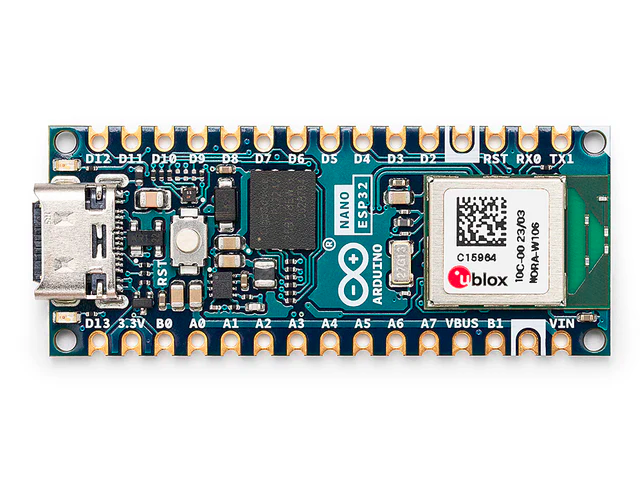
\includegraphics[scale=0.30]{img/arduino.png}
	\caption{Arduino Nano ESP32}
	\footnotesize{Arduino, licencované pod \href{https://creativecommons.org/licenses/by-sa/4.0/deed.en}{CC BY-SA 4.0}, cez arduino.cc.}
	\label{fig:arduino}
\end{figure}
\noindent\textbf{Technické parametre:}
\begin{itemize}
	\item Rozmery: 18 * 45mm
	\item Vstupné/výstupné napätie: 3.3V
	\item Počet \acrshort{gpio} pinov: 48
	\item Komunikačné rozhrania: UART, I2C, SPI
	\item Rýchlosť procesora: 240Mhz
	\item Veľkosť ROM: 384kB
	\item Veľkosť S\acrshort{ram}: 512kB
	\item Veľkosť \acrshort{ram}: 8MB
\end{itemize}
\subsection{ESP32-CAM + OV2640 kamera}
Vývojová doska ESP32-CAM integruje Wi-Fi a Bluetooth modul spolu s rozhraním na pripojenie 2MPx kamerový senzor OV2640. Táto kombinácia nám poskytuje oddelenú implementáciu prenosu videa, čím uvolníme výpočtovú záťaž hlavného čipu. Senzor OV2640 disponuje s natívnym rozlíšením 1600 x 1200 pixelov a obrazovou frekvenciou 60 FPS, čo poskytuje dostatočnú výkonovú rezervu~\cite{esp32cam}\cite{ov2640}.\par
\begin{figure}[!ht]
	\centering
	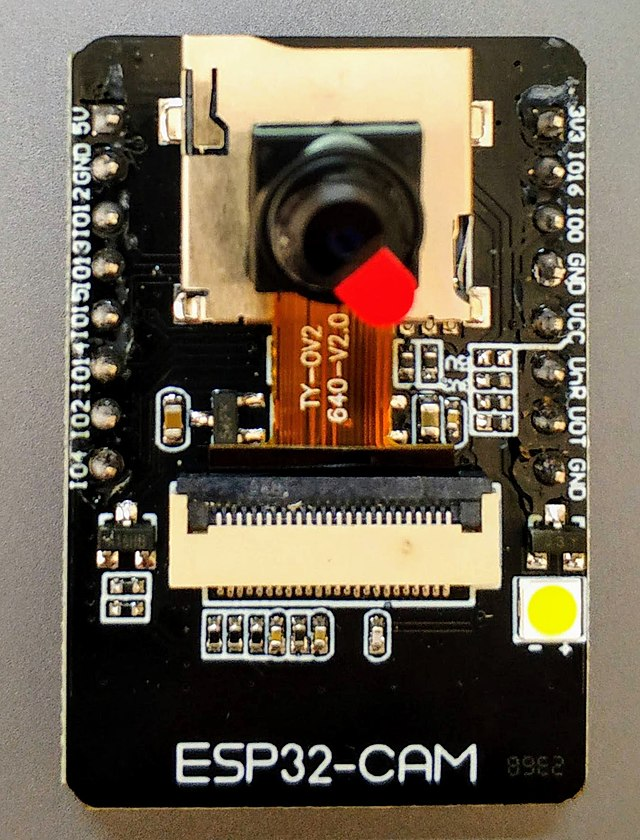
\includegraphics[scale=0.20]{img/esp32cam.jpg}
	\caption{ESP32-CAM a OV2640}
	\footnotesize{Nowforever, licencované pod \href{https://creativecommons.org/licenses/by-sa/4.0/deed.en}{CC BY-SA 4.0}, cez Wikimedia Commons.}
	\label{fig:esp32cam}
\end{figure}
\noindent\textbf{Technické parametre:}
\begin{itemize}
	\item Rozmery: 27 * 40mm
	\item Pracovné napätie: 2.2V - 3.6V
	\item Rozlíšenie kamery: 1600 x 1200
	\item Frame rate kamery: 60FPS (pri CIF formáte)
	\item Rýchlosť procesora: 240Mhz
	\item Veľkosť FLASH: 4MB
	\item Veľkosť PS\acrshort{ram}: 4MB
\end{itemize}
\subsection{HC-SR04 Ultrazvukový senzor}
Ultrazvukový senzor je zariadenie, ktoré generuje a deteguje ultrazvukové vlny. Tieto vlny sa odrazia od objektu a vrátia sa k prijímaču. Meraním času, za ktorý sa vlna vráti a znalosť rýchlosti zvuku dokážeme určiť vzdialenosť objektu.\par
HC-SR04 je nákladovo efektívne riešenie na detekciu prekážky pred vozidlom. Používame ho ako sekundárny systém na núdzové zastavenie vozidla v prípade, že kamerový systém nedetekuje prekážku~\cite{hcsr04}.\par
\begin{figure}[!ht]
	\centering
	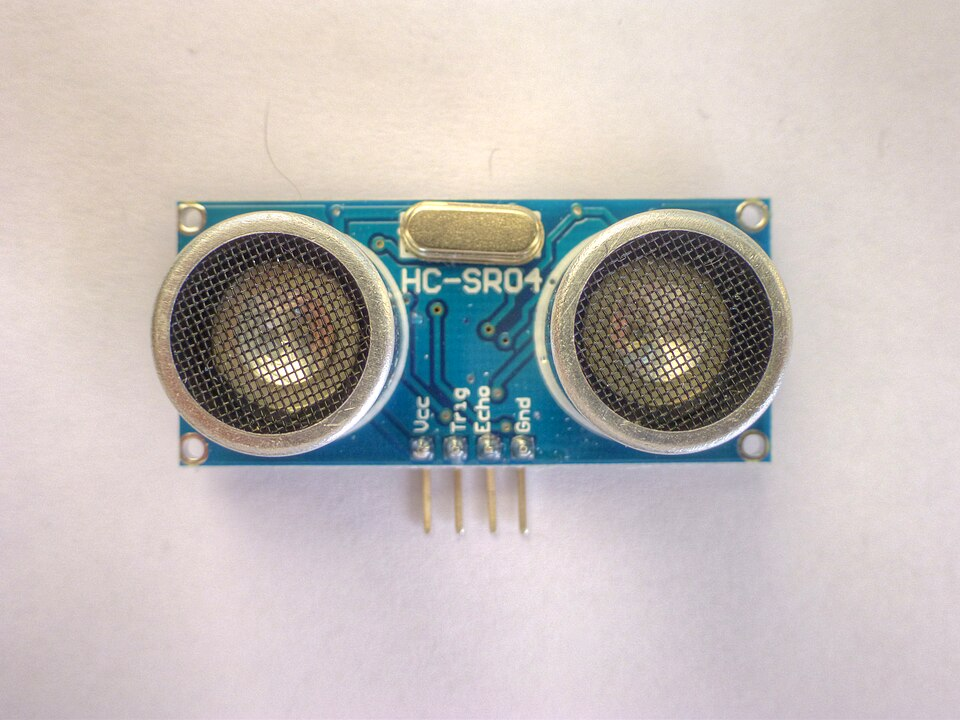
\includegraphics[scale=0.20]{img/hcsr04.jpg}
	\caption{HC-SR04 Ultrazvukový senzor}
	\footnotesize{Nevit Dilmen, licencované pod \href{https://creativecommons.org/licenses/by-sa/3.0/deed.en}{CC BY-SA 3.0}, cez Wikimedia Commons.}
	\label{fig:hcsr04}
\end{figure}
\noindent\textbf{Technické parametre:}
\begin{itemize}
	\item Rozmery: 20 * 45 * 15mm
	\item Pracovné napätie: 5V
	\item Maximálna vzdialenosť: 4n
	\item Minimálna vzdialenosť: 2cm
	\item Merací úhol: 15°
\end{itemize}
\subsection{DRV8833 driver pre motorčeky}
Motor driver je zariadenie určené na riadenie motorov. Slúži na zosilnenie slabého signálu z riadiacej jednotky (napr. mikrokontroléra), aby motoru poskytol potrebné napätie a prúd. Mnohé moduly poskytujú možnosť ovládať rýchlosť aj smer otáčania motorov.\par
DRV8833 sme použili na nezávislé riadenie dvoch \acrshort{dc} motorov. Integrovaný obvod obsahuje dvojitý H-mostík, ktorý umožnuje meniť polaritu napätia, a tým aj smer otáčania motorov. Modul má štyri vstupné piny (dva pre každý motor), pomocou ktorých možno ovládať rýchlosť a smer otáčania~\cite{drv8833}.\par
\begin{figure}[!ht]
	\centering
	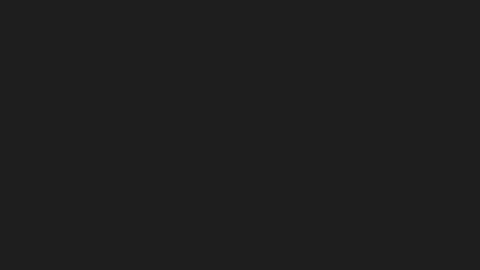
\includegraphics[scale=0.20]{img/drv8833.png}
	\caption{DRV8833 driver pre motorčeky}
	\footnotesize{vlastná fotografia.}
	\label{fig:drv8833}
\end{figure}
\noindent\textbf{Technické parametre:}
\begin{itemize}
	\item Rozmery: 5 * 4 mm
	\item Logické napätie: 2.7V - 10.8V
	\item Drive napätie: 3V - 10V
	\item Drive prúd: 1.5A (MAX pre jeden mostík)
	\item Maximálny výkon: 15W
\end{itemize}
\subsection{Ďalšie elektrické komponenty}
V implementácií sme použili Li-Ion akumulátor s napätím 7.4V a kapacitou 1500mAh. Pohon zabezpečujú dva \acrshort{dc} motorčeky s prevodovkou na 200\acrshort{rpm} pri 3V. Kvôli ochrane komponentov vyžadujúce 5V napájanie sme do systému zapojili menič napätia (step-down buck converter). Súčasťou zapojenia je taktiež kolískový prepínač na vypnutie/zapnutie systému.
\subsection{Server}
Server je počítač alebo softvér, ktorý poskytuje dáta, zdroje alebo služby iným počítačom. Táto architektúra sa nazýva klient-server model, kde server je podradený klientovi.\par
Vzhľadom na obmedzený výpočtový výkon mikrokontrolérov Arduino, ktoré nie sú schopné vykonávať komplexné výpočty neurónových sietí v reálnom čase, sme do systému zaradili centrálny server. Ten zabezpečuje spracovanie obrazu a koordináciu bezdrótových periférií. V našej implementácii túto úlohu plní laptop, ktorý zároveň slúži ako prístupový bod pre Wi-Fi sieť.

\section{Softvér}\label{sec:Softver}
V nasledovnej časti sa oboznámime s použitým softvérom, ktorý nám umožnuje preklad požiadaviek systému na skutočné inštrukcie vykonateľné hardvérom.
\subsection{C++}
C++ je programovací jazyk vyššej úrovne na všeobecné použitie, ktorý umožnuje pracovať s prostriedkami nízkej úrovne. Bjarne Stroustrup vyvinul C++ v roku 1983 ako rozšírenie jazyka C~\cite{stroustrupcpp}.\par
Mikrokontroléry Arduino je možné programovať pomocou jazykov C/C++ vďaka štandardnému \glslink{api}{rozhraniu pre programovanie aplikácií} (\acrshort{api}) známemu ako Arduino Programming Language. Toto \acrshort{api} obsahuje funkcie a knižnice na ovládanie hardvéru mikrokontroléra. Projekt Arduino taktiež poskytuje vývojové prostredie Arduino \acrshort{ide}, v ktorom je kompilácia, integrácia knižníc a nahrávanie kódu zjednodušené.\par
V našej implementácii používame C++ pre programovanie nízkoúrovňového mikrokontroléru Arduino Nano ESP32 a kamerového modulu ESP32-CAM.
\subsection{Python}
Python je interpretovaný, interaktívny programovací jazyk vysokej úrovne, ktorý vytvoril Guido van Rossum. Je dynamicky typovaný, čo znamená, že typ premennej sa určuje za behu programu. Na rozdiel od jazykov C/C++, využíva Garbage Collection, vďaka čomu programátor nemusí manuálne riešiť alokovanie a uvolňovanie pamäte. Štruktúra kódu je definovaná odsadením, čím sa výrazne zvyšuje čitateľnosť kódu~\cite{kuhlmanpython}.\par
V súčasnosti je Python populárnou voľbou v oblasti umelej inteligencie, vďaka jeho jednoduchosti a rozširenej podpore knižníc pre prácu s neurónovými sieťami. Hoci je Python ako jazyk pomalší, pri vývoji \acrshort{ai} to nepredstavuje prekážku, keďže kritické výpočty sú vykonávané nízkoúrovňovým kódom optimalizovaným pre \acrshort{cpu} a \acrshort{gpu}.\par
V našej implementácii používame Python na vytvorenie Wi-Fi servera, spracovanie dát z kamery a následnú interpretáciu výsledkov do podoby príkazov pre pohyb kolies.
\subsection{OpenCV}
OpenCV je knižnica programovacích funkcií určených na počítačové videnie v reálnom čase, ktorú pôvodne vyvinula spoločnosť Intel. Využíva sa v oblastiach detekcie objektov, tvárí a gest, pri vizuálnej odometrii, vnímaní hĺbky či v augmentovanej realite. Knižnica OpenCV je napísaná v programovacom jazyku C++, no ponúka rozhrania pre integráciu v ďalších jazykoch, ako sú Python, Java alebo MATLAB~\cite{acm2012}\cite{opencv2025}.\par
V našej implementácii používame OpenCV na detekciu vozovky a analýzu jazdných pruhov.
\subsection{Ultralytics YOLOv8}
YOLOv8 je model umelej inteligencie od spoločnosti Ultralytics určený na detekciu objektov v reálnom čase. Tento model je založený na \glslink{cnn}{konvolučných neurónových sietí} (\acrshort{cnn}), čo je typ dopredných neurónových sietí, ktoré využívajú matematickú konvolúciu na učenie vzorov zo vstupu. Model \acrfull{yolo} vyžaduje iba jednu doprednú propagáciu (forward pass) na vytvorenie predpokladu. Pre programovací jazyk Python existuje jednoduché rozhranie, ktoré prácu s modelom zjednodušuje~\cite{make2023}\cite{yolo2023}.\par
Tento model je už predtrénovaný na rozsiahlych datasetoch, vďaka čomu je pripravený na okamžitú implementáciu bez nutnosti zložitej konfigurácie. V našej implementácii ho využívame na detekciu prekážky v dráhe vozidla.

\section{Návrh a implementácia}\label{sec:NavrhAImplementacia}
Vhodný návrh architektúry je kľúčový pre efektívnu spoluprácu všetkých komponentov. Počas vývoja bolo otestovaných niekoľko prístupov, kým sa nepodarilo dosiahnuť optimálne riešenie. V tejto kapitole popíšeme použitý dizajn a jeho následnú implementáciu.
\subsection{Návrh komunikácie komponentov}
Komunikácia komponentov predstavuje dôležitý aspekt projektu, pretože je nutné aby si jednotlivé časti mohli synchrónne vymieňať a spracovať dáta. Systém je navrhnutý tak, aby v prípade výpadku jedného alebo viacerých komponentov dokázal bezpečne zastaviť vozidlo.\par
Dôsledkom nízkeho výpočtového výkonu mikrokontrolérov Arduino sme použili v našej implementácii model klient-server. V danej štruktúre vystupujú dva typy entít; nadradení klienti iniciujú požiadavky na pasívny server, ktorý posiela odpovede klientom.\par
\begin{figure}[!ht]
	\centering
	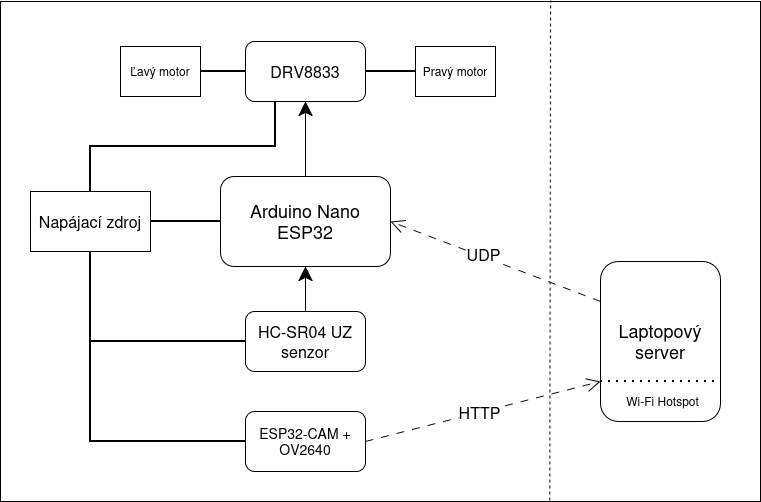
\includegraphics[scale=0.50]{img/diagram1.png}
	\caption{Diagram komunikácie komponentov}
	\footnotesize{vlastný diagram.}
	\label{fig:spojenie}
\end{figure}
Server je v našom projekte laptop, ktorý taktiež spúšťa Wi-Fi sieť na komunikáciu s komponentmi. Všetky funkcie webserveru sme programovali pomocou jazyka Python. Bezdrôtový pripojný bod sme vytvorili NetworkManagerom, nástrojom na konfiguráciu sieťových zariadení v operačnom systéme Linux, pomocou ktorého sme sieťovú kartu našeho laptopu zmenili na prípojný bod Wi-Fi hotspotu. Na spustenie tohto programu v Pythone sme použili knižnicu subprocess. \par
\lstset{style=code}
\begin{lstlisting}[language=Python, caption=Zapnutie Wi-Fi hotspotu]
import subprocess
import socket

SSID = "LAPTOP_AP"
PASSWORD = "12345678"

def startHotspot():
    print("Starting Hotspot")
    subprocess.run([
        "nmcli",
        "device",
        "wifi",
        "hotspot",
        "ssid", SSID,
        "password", PASSWORD
    ], check=True)
\end{lstlisting}
ESP32-CAM pracuje ako klient, ktorý posiela obrázkové dáta na server za pomoci Wi-Fi. Po pripojení na server začne cez protokol HTTP na porte 81 vysielať video z kamery OV2640. Obrázky sú rozlíšenia QVGA (t.j 320x240 pixelov) s formátom JPEG. Nový obrázok sa pošle každých 30ms, čo znamená, že stream má približne 30FPS.\par
\begin{lstlisting}[language=C++, caption=Spustenie HTTP stream na ESP32-CAM]
void startCameraServer(){
  httpd_config_t config = HTTPD_DEFAULT_CONFIG();
  config.server_port = 81; // port streamu

  if(httpd_start(&stream_httpd, &config) == ESP_OK){
    httpd_uri_t stream_uri = {
      .uri       = "/stream",
      .method    = HTTP_GET,
      .handler   = stream_handler,
      .user_ctx  = NULL
    };
    httpd_register_uri_handler(stream_httpd, &stream_uri);
  }
}
\end{lstlisting}
Vďaka statickej IP adrese dokážeme serveru povedať na akej URL má očakávať obrázky. Funkcia VideoCapture z knižnice OpenCV má podporu pre spracovanie obrazu z URL. Po interpretovaní dát, server pošle požiadavku na Arduino Nano. Odpoveď sa odošle cez UDP socket, ideálne pre aplikácie fungujúce v reálnom čase, IP adrese mikrokontroléra na porte 5005. Komunikáciu sprostredkuje Python knižnica socket. Poslané dáta sú vo forme 2 bytov, čo je najmenší potrebný buffer na uloženie údajov o riadení.\par
\begin{lstlisting}[language=Python, caption=Posielanie UDP packetov]
import struct

CAM_IP = "10.42.0.128"
CAM_URL = "http://10.42.0.128:81/stream"

UDP_IP = "10.42.0.111"
UDP_PORT = 5005

sock = socket.socket(socket.AF_INET, socket.SOCK_DGRAM)

def sendUDP(direction: float):
    sock.sendto(struct.pack('<H', direction), (UDP_IP, UDP_PORT))
\end{lstlisting}
Arduino príjme UDP packet a súčasne získa nameránu vzdialenosť z ultrazvukového senzora. Snímač sa spúšťa v intervaloch 50ms, z dôvodu efektívneho využitia výpočtového výkonu. Ak vyhodnotí, že objekt pred senzorom je do 10 cm, vozidlo zastaví, inak nastaví riadenie motorov. Každému z motorčekov sú priradené dva výstupné piny -- pulse width modulation (PWM) a smerový (DIR) pin. PWM riadi rýchlosť a DIR smer otáčania kolies. Signály z pinov sú zaslané na DRV8833, ktorý fyzicky poháňa dva \acrshort{dc} motory.
\begin{lstlisting}[language=C++, caption=Vnútorný cyklus Arduina]
void loop() {
  while (udp.parsePacket() >= 2) {
    udp.read(incoming, 2);

    uint16_t raw = incoming[0] | (incoming[1] << 8);
    steer = (int)raw - 256;
  }

  static unsigned long lastTrig = 0;
  if (millis() - lastTrig > 50) {
    lastTrig = millis();
    echoDone = false;
    triggerUltrasonic();
  }

  if (echoDone) {
    uint32_t duration = echoEnd - echoStart;
    distance = duration / 58;
    echoDone = false;
  }

  if (distance < 10 || steer < -255 || steer > 255) {
    stopWheels();
  } else {
    driveSteering(steer*2);
  }
}
\end{lstlisting}
\subsection{Návrh rámu a rozloženie komponentov}
Správny návrh rámu a rozloženia komponentov na ňom je doležité pre správne fungovanie celého systému. V našej implementácii sme sa zamerali na minimalizovanie váhy vozidla a maximalizovanie kompaktnosti komponentov a tým ich zohranie.\par
Na návrh rámu sme použili softvér Blender, populárny všeobecne používaný program na dizajn, modelovanie a animáciu, ktorý je taktiež schopný exportovať vo formáte '.stl', ideálny pre 3D tlač. Po odmeraní všetkých komponetov, sme začali pracovať na prototypu rámu. Vyskúšali sme mnoho návrhov, kde sme otestovali rôzne rozloženia a orientácie komponentov. Vybrali sme si dvojkolesový dizajn vpredu so zadnou vidlicou, ktorá sa dá vymeniť (v prípade opotrebovania alebo zmeny povrchu). Najťažšie komponenty -- batériu a menič napätia -- sme umiestnili na spodok vozidla pre zníženie ťažiška a zvýšenie stability. Pridali sme držiak na kameru a ultrazvukový senzor na stabilizovanie obrazu. Kolesá sme navrhli ako duté valce na minimalizovanie váhy.\par
Model bol vytlačený na tlačiarni Bambulab A1 Mini, použitím filamentu kyseliny polymliečnej (PLA). Podobne sme pre kolesá vozidla využili odolnejšiu náplň polyetyléntereftálatu modifikovaného glykolom (PETG).\par
\subsection{Montovanie vozidla}
Po získaní všetkých potrebných komponentov sme začali s montovaním vozidla. Na prepojenie komponentov sme použili nepájivé pole a farebne odlíšené kábliky. Podľa definície pinov v kóde sme dokopy zapojili jednotlivé elektronické prvky. Na rám vozidla sme pripevnili nepájivé pole pomocou adhezívneho prvku na jeho spodku.

\section{Detekcia vozovky}\label{sec:DetekciaVozovky}
\subsection{Region of interest}
\subsection{Hľadanie svetlých regiónov}
\subsection{Hľadanie kontúr vozovky}
\subsection{Interpretácia dát}

\section{Detekcia prekážky}\label{sec:DetekciaPrekazky}
\subsection{Ultrazvukový senzor}
\subsection{CNN}
\subsection{Interpretácia dát}

\section{Metodika a testovanie}\label{sec:MetodikaATestovanie}
\subsection{Metodika}
\subsection{Testovanie}

\section{Výsledky}\label{sec:Vysledky}
